\subsection{Preprocesamiento de los datos experimentales}

Un procedimiento experimental usual para evaluar los materiales de las baterías
consiste en medir los perfiles galvanostáticos a distintos valores de C-rate.
En la Figura \ref{fig:preproc} se muestran como ejemplo las mediciones realizadas
por Wang \textit{et al.} \cite{wang2019high} para LiCoO$_2$ (LCO) recubierto con 
TiO$_2$. Además, se agrega una línea punteada horizontal que se corresponde
con el potencial de equilibrio reportado en el trabajo citado, 3.9 V, y otra
0.15 V por debajo, que es el valor que corresponde al potencial de corte
elegido en este capítulo. Esta es la región de interés en el gráfico, ya que 
los valores en los que el SOC se intersecta con esta última curva (SOC$_{\max}$)
son los que se utilizan para ajustar el modelo en función de C-rate.
\begin{figure}[h!]
    \centering
    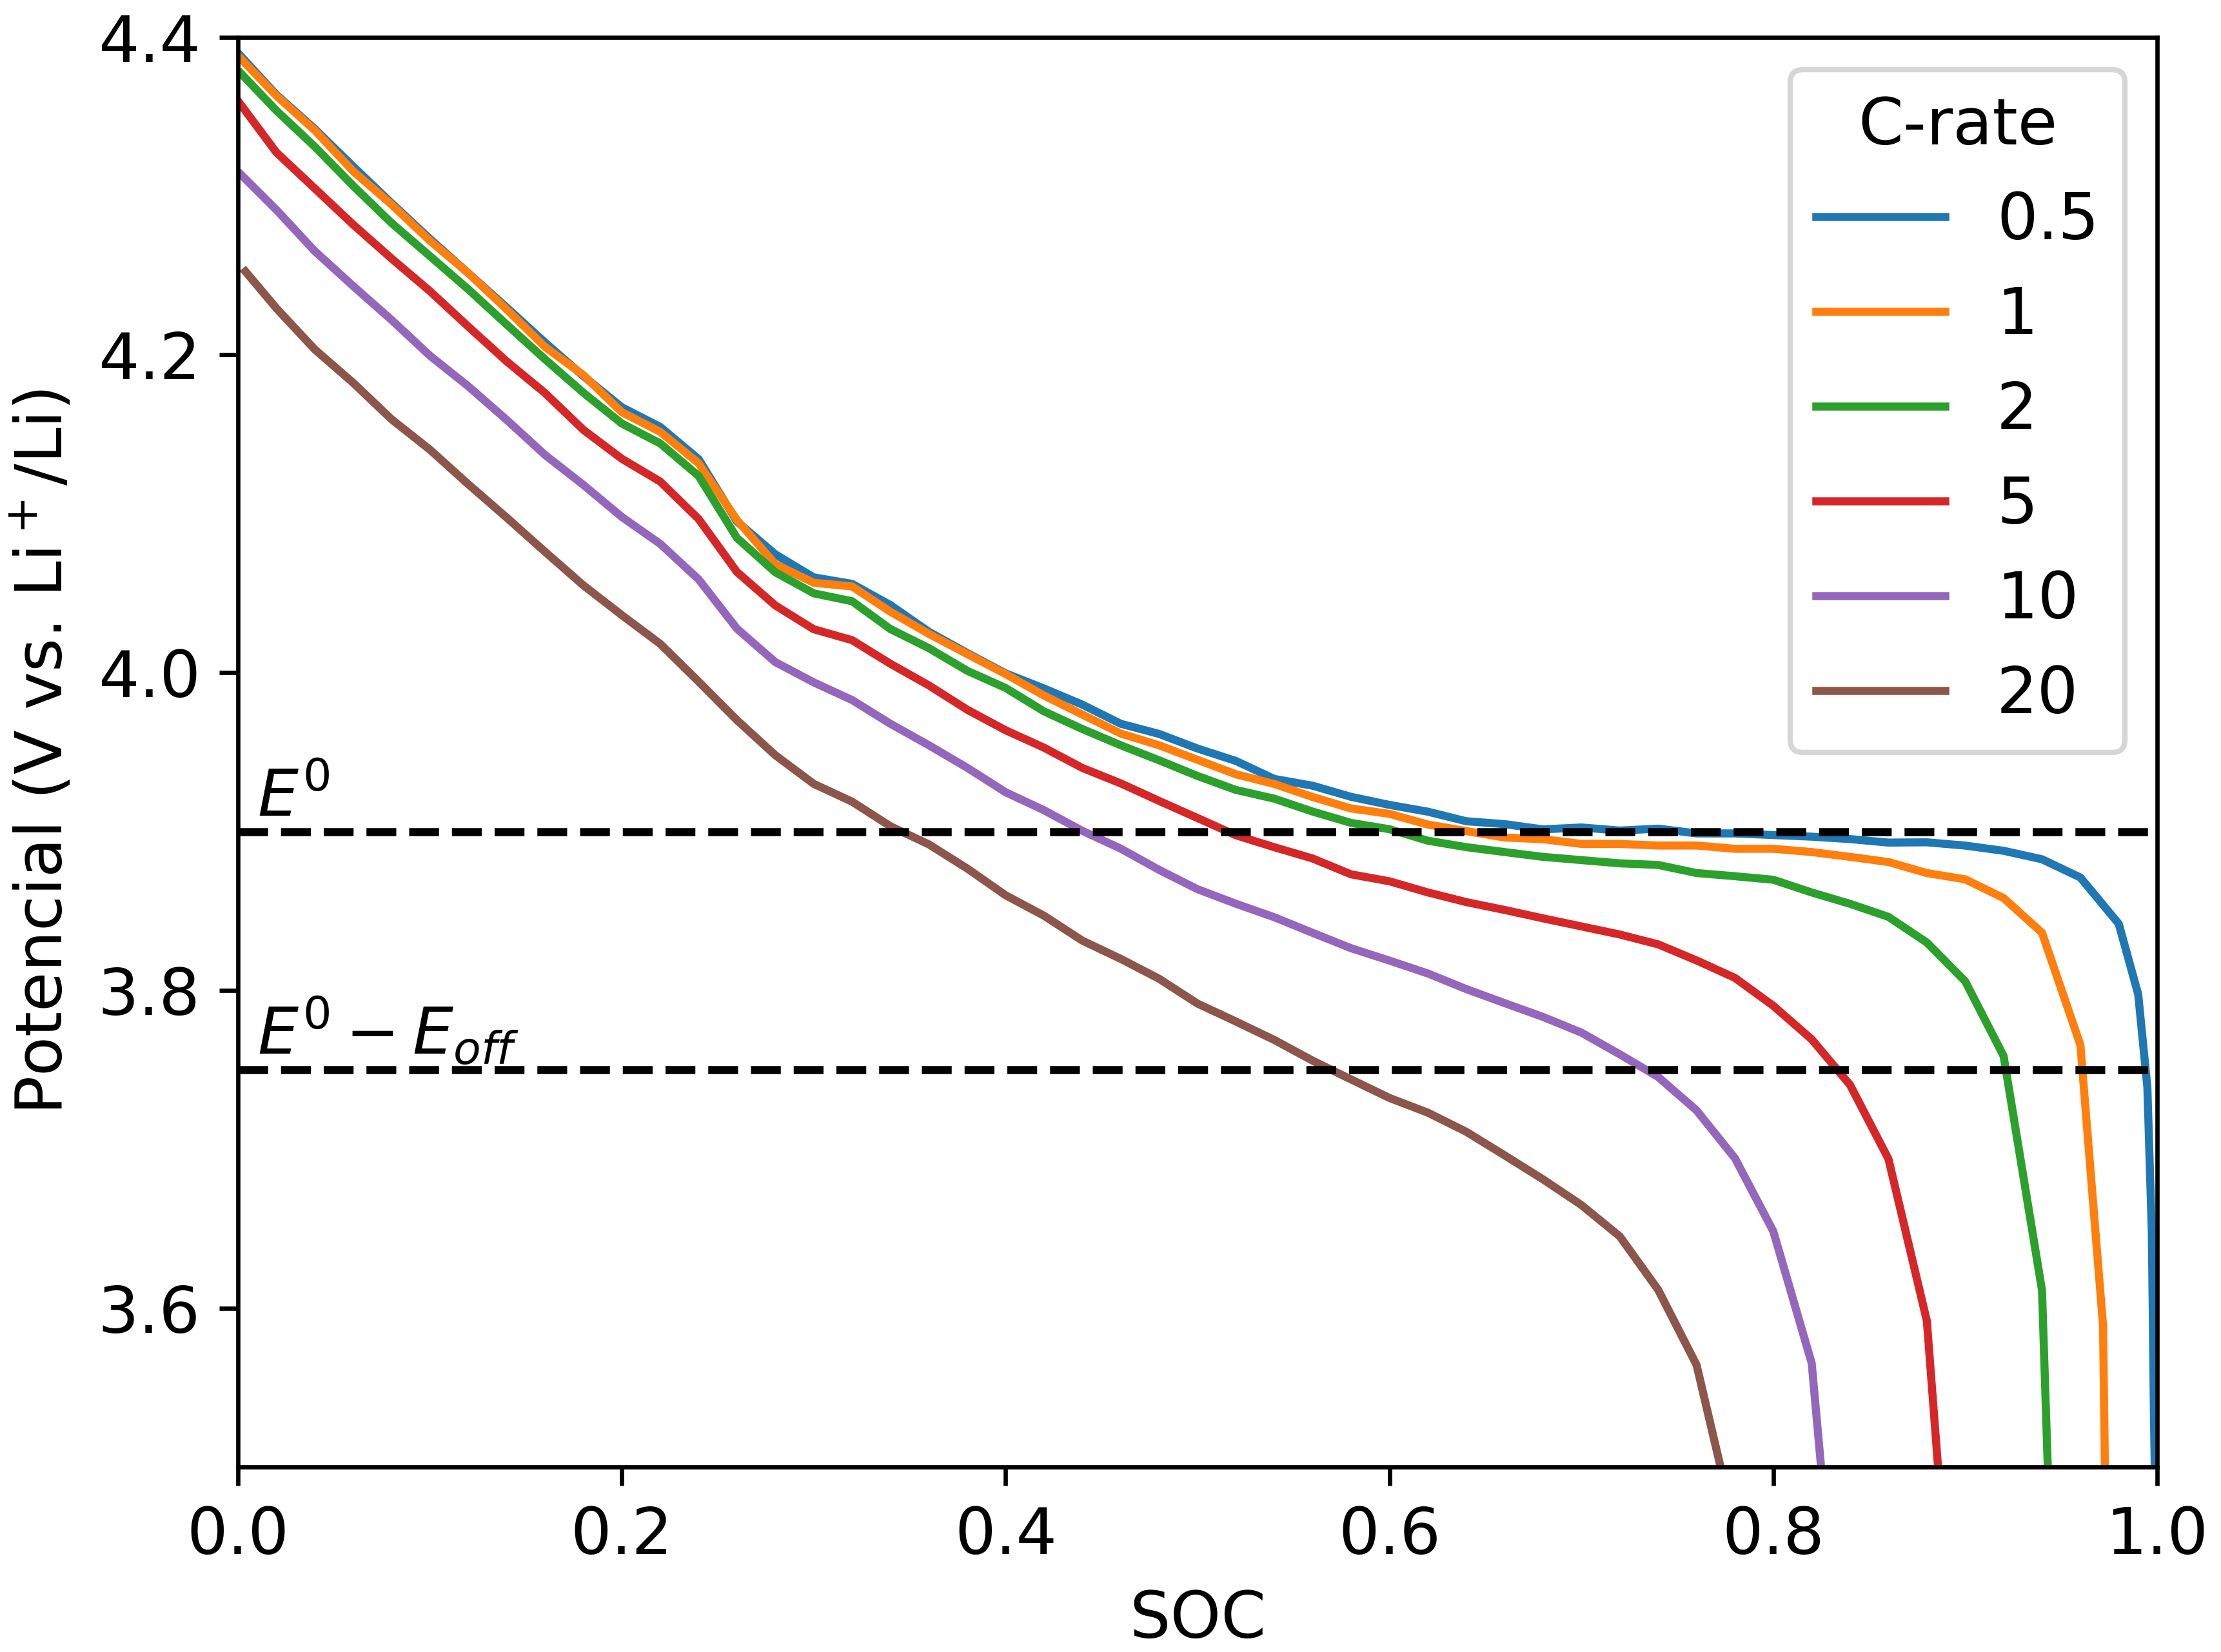
\includegraphics[width=0.7\textwidth]{FastCharging/un/resultados/preprocesamiento/preprocesamiento.png}
    \caption{Perfiles galvanostáticos para distintos valores de C-rate para el
    sistema LCO recubierto de TiO$_2$. Las líneas horizontales indican el 
    potencial de equilibrio y el de corte utilizado para determinar la 
    capacidad máxima normalizada alcanzada (SOC$_{\max}$) a cada C-rate. 
    Reproducido del trabajo de Wang \textit{et al.} \cite{wang2019high}.}
    \label{fig:preproc}
\end{figure}

Es importante destacar que, en el trabajo citado, los perfiles galvanostáticos
se presentan en función del SOC normalizado, que no siempre es el caso. La 
forma usual en la que estos resultados son reportados es en función de la 
capacidad de descarga. En estos casos, es necesario normalizarla con respecto
a la capacidad máxima ($Q_{\max}$) alcanzada por el material, para así obtener
el SOC normalizado. El criterio utilizado en este capítulo para encontrar 
$Q_{\max}$ fue considerar el valor máximo de la capacidad alcanzado por la 
medición a la C-rate más baja. Gráficos similares al presentado en la Figura 
\ref{fig:preproc} son obtenidos en el resto de los trabajos experimentales que
se utilizan en los ajustes que siguen.
